%\documentclass[11pt,oneside,a4paper,openright]{report}
%\usepackage[utf8]{inputenc}
%\renewcommand{\contentsname}{Indholdsfortegnelse}
%\usepackage{pdfpages}
%\usepackage{titlesec}
%\titleformat{\chapter}{\normalfont\huge}{\thechapter.}{20pt}{\huge\it}

%%%% Dokumentklassen %%%%

\documentclass[a4paper,11pt,dvipsnames,oneside,openany]{memoir} 	% Openright åbner kapitler på højresider (openany begge)
% fleqn = flush left equation - sikre at alle ligninger tvinges til venstre. I 3. semesterprojektet, skulle ligningerne stå i midten derfor er denne pakke slettet fra dokumentklassen.

\usepackage{subfiles}
\usepackage{nameref}
\usepackage{tabularx}
\usepackage{multirow}
\usepackage[table]{xcolor}


%%%% PACKAGES %%%%

%% Oversættelse og tegnsætning %%
\usepackage[utf8]{inputenc}					% Input-indkodning af tegnsæt (UTF8)
\usepackage[danish]{babel}					% Dokumentets sprog
\usepackage[T1]{fontenc}				    % Output-indkodning af tegnsæt (T1)
\usepackage{ragged2e,anyfontsize}			% Justering af elementer
%\usepackage{fixltx2e}						% Retter forskellige fejl i LaTeX-kernen
\usepackage{titletoc}
\newcommand{\nocontentsline}[3]{}
\newcommand{\tocless}[2]{\bgroup\let\addcontentsline=\nocontentsline#1{#2}\egroup}									% Giver mulighed for at fjerne section nummer i indholdsfortegnelse ved \tocless


\usepackage{lastpage}						% Total antal sider opdateres automatisk ved \pageref{LastPage}
\usepackage{tikz}							% Til at lave flow diagrammer
\usetikzlibrary{calc,trees,positioning,arrows,chains,shapes.geometric,decorations.pathreplacing,decorations.pathmorphing,shapes,matrix,shapes.symbols}				% Til at lave diagrammer
																			
%% Figurer og tabeller (floats) %%
\usepackage{graphicx} 						% Håndtering af eksterne billeder (JPG, PNG, EPS, PDF)
\usepackage{multicol}         	           	% Muliggør output i spalter
\usepackage{rotating}						% Rotation af tekst med \begin{sideways}...\end{sideways}
\usepackage{xcolor}							% Definer farver med \definecolor. Se mere: http://en.wikibooks.org/wiki/LaTeX/Colors
\usepackage{flafter}						% Sørger for at floats ikke optræder i teksten før deres reference
\let\newfloat\relax 						% Justering mellem float-pakken og memoir
\usepackage{float}							% Muliggør eksakt placering af floats, f.eks. \begin{figure}[H]
\usepackage{color, colortbl}				% Tilføjer farve til tabeller

\definecolor{Gray}{gray}{0.9}				% Definerer en farve "yeezy-gray"

%% Matematik mm. %%
\usepackage{amsmath,amssymb,stmaryrd} 		% Avancerede matematik-udvidelser
\usepackage{mathtools}						% Andre matematik- og tegnudvidelser
\usepackage{textcomp}                 		% Symbol-udvidelser (fx promille-tegn med \textperthousand)
\usepackage{rsphrase}						% Kemi-pakke til RS-saetninger, fx \rsphrase{R1}
\usepackage[version=3]{mhchem} 				% Kemi-pakke til flot og let notation af formler, f.eks. \ce{Fe2O3}
\usepackage{siunitx}						% Flot og konsistent præsentation af tal og enheder med \si{enhed} og \SI{tal}{enhed}
\sisetup{output-decimal-marker = {,}}		% Opsætning af \SI (DE for komma som decimalseparator) 

%% Referencer og kilder %%
\usepackage[danish]{varioref}				% Muliggør bl.a. krydshenvisninger med sidetal (\vref)
\usepackage{natbib}							% Udvidelse med naturvidenskabelige citationsmodeller
\usepackage{xr}							    % Referencer til eksternt dokument med \externaldocument{<NAVN>}

%% Misc. %%
\usepackage{listings}						% Placer kildekode i dokumentet med \begin{lstlisting}...\end{lstlisting}
\usepackage{lipsum}							% Dummy text \lipsum[..]
\usepackage[shortlabels]{enumitem}			% Muliggør enkelt konfiguration af lister
\usepackage{pdfpages}						% Gør det muligt at inkludere pdf-dokumenter med kommandoen \includepdf[pages={x-y}]{fil.pdf}	
\pdfoptionpdfminorversion=6					% Muliggør inkludering af pdf-dokumenter, af version 1.6 og højere
\pretolerance=2500 							% Justering af afstand mellem ord (højt tal, mindre orddeling og mere luft mellem ord)


%%%% CUSTOM SETTINGS %%%%

%% Marginer %%
\setlrmarginsandblock{3.0cm}{3.0cm}{*}		% \setlrmarginsandblock{Indbinding}{Kant}{Ratio}
\setulmarginsandblock{3.0cm}{3.0cm}{*}		% \setulmarginsandblock{Top}{Bund}{Ratio}
\checkandfixthelayout 						% Oversætter værdier til brug for andre pakker

%% Afsnitsformatering %%
\setlength{\parindent}{0mm}           		% Størrelse af indryk
\setlength{\parskip}{3mm}          			% Afstand mellem afsnit ved brug af double Enter
\linespread{1,1}							% Linjeafstand

%% Indholdsfortegnelse %%
\setsecnumdepth{subsection}		 			% Dybden af nummererede overskrifter (part/chapter/section/subsection)
\maxsecnumdepth{subsection}					% Dokumentklassens grænse for nummereringsdybde
\settocdepth{subsubsection} 					% Dybden af indholdsfortegnelsen
\setcounter{secnumdepth}{5} 				    % Ekstra subsubsection nummerering
		
%% Opsætning af listings %%
\definecolor{commentGreen}{RGB}{34,139,24}
\definecolor{stringPurple}{RGB}{208,76,239}

\lstset{language=Matlab,				    % Sprog
	basicstyle=\ttfamily\scriptsize,	    % Opsætning af teksten
	keywords={for,if,while,else,elseif,		% Nøgleord at fremhæve
			  end,break,return,case,
			  switch,function},
	keywordstyle=\color{blue},				% Opsætning af nøgleord
	commentstyle=\color{commentGreen},		% Opsætning af kommentarer
	stringstyle=\color{stringPurple},		% Opsætning af strenge
	showstringspaces=false,					% Mellemrum i strenge enten vist eller blanke
	numbers=left, numberstyle=\tiny,		    % Linjenumre
	extendedchars=true, 					    % Tillader specielle karakterer
	columns=flexible,						% Kolonnejustering
	breaklines, breakatwhitespace=true,		% Bryd lange linjer
}

%% Navngivning %%
\addto\captionsdanish{
	\renewcommand\appendixname{Appendiks}
	\renewcommand\contentsname{Indholdsfortegnelse}	
	\renewcommand\appendixpagename{Appendiks}
	\renewcommand\appendixtocname{Appendiks}
	\renewcommand\cftchaptername{\chaptername~}		% Skriver "Kapitel" foran kapitlerne i indholdsfortegnelsen
	\renewcommand\cftappendixname{\appendixname~}	% Skriver "Appendiks" foran appendiks i indholdsfortegnelsen
}

%% Kapiteludssende %%
\definecolor{numbercolor}{gray}{0.7}		            % Definerer en farve til brug til kapiteludseende
\newif\ifchapternonum

\makechapterstyle{jenor}{					        % Definerer kapiteludseende frem til ...
  \renewcommand\beforechapskip{0pt}
  \renewcommand\printchaptername{}
  \renewcommand\printchapternum{}
  \renewcommand\printchapternonum{\chapternonumtrue}
  \renewcommand\chaptitlefont{\fontfamily{pbk}\fontseries{db}\fontshape{n}\fontsize{25}{35}\selectfont\raggedleft}
  \renewcommand\chapnumfont{\fontfamily{pbk}\fontseries{m}\fontshape{n}\fontsize{1in}{0in}\selectfont\color{numbercolor}}
  \renewcommand\printchaptertitle[1]{%
    \noindent
    \ifchapternonum
    \begin{tabularx}{\textwidth}{X}
    {\let\\\newline\chaptitlefont ##1\par} 
    \end{tabularx}
    \par\vskip-2.5mm\hrule
    \else
    \begin{tabularx}{\textwidth}{Xl}
    {\parbox[b]{\linewidth}{\chaptitlefont ##1}} & \raisebox{-15pt}{\chapnumfont \thechapter}
    \end{tabularx}
    \par\vskip2mm\hrule
    \fi
  }
}											        % ... her

\chapterstyle{jenor}						        % Valg af kapiteludseende - Google 'memoir chapter styles' for alternativer

%% Sidehoved %%

\makepagestyle{AAU}							        % Definerer sidehoved og sidefod udseende frem til ...
\makepsmarks{AAU}{%
	\createmark{chapter}{left}{shownumber}{}{. \ }
	\createmark{section}{right}{shownumber}{}{. \ }
	\createplainmark{toc}{both}{\contentsname}
	\createplainmark{lof}{both}{\listfigurename}
	\createplainmark{lot}{both}{\listtablename}
	\createplainmark{bib}{both}{\bibname}
	\createplainmark{index}{both}{\indexname}
	\createplainmark{glossary}{both}{\glossaryname}
}
\nouppercaseheads									% Ingen Caps ønskes

\makeevenhead{AAU}{\small E17BAC-Synk2}{}{\leftmark}	% Definerer lige siders sidehoved (\makeevenhead{Navn}{Venstre}{Center}{Hoejre})
\makeoddhead{AAU}{\rightmark}{}{}		            % Definerer ulige siders sidehoved (\makeoddhead{Navn}{Venstre}{Center}{Højre})
\makeevenfoot{AAU}{\small \thepage \ }{}{ }						% Definerer lige siders sidefod (\makeevenfoot{Navn}{Venstre}{Center}{Højre})
\makeoddfoot{AAU}{}{}{\small \thepage \ }						% Definerer ulige siders sidefod (\makeoddfoot{Navn}{Venstre}{Center}{Højre})

\copypagestyle{AAUchap}{AAU}							% Sidehoved for kapitelsider defineres som standardsider, men med blank sidehoved
\makeoddhead{AAUchap}{}{}{}
\makeevenhead{AAUchap}{}{}{}
\makeheadrule{AAUchap}{\textwidth}{0pt}
\aliaspagestyle{chapter}{AAUchap}					% Den ny style vælges til at gælde for chapters
													% ... her
															
\pagestyle{AAU}										% Valg af sidehoved og sidefod


%%%% CUSTOM COMMANDS %%%%

%% Billede hack %%
\newcommand{\figur}[4]{
		\begin{figure}[H] \centering
			\includegraphics[width=#1\textwidth]{billeder/#2}
			\caption{#3}\label{#4}
		\end{figure} 
}

%% Specielle tegn %%
\newcommand{\decC}{^{\circ}\text{C}}
\newcommand{\dec}{^{\circ}}
\newcommand{\m}{\cdot}


%%%% ORDDELING %%%%

\hyphenation{}


%%%% Tilføjelser af min preample %%%%

% Booktabs:
% The booktabs package is needed for better looking tables. 
\usepackage{booktabs}

% Caption:
% For better looking captions. See caption documentation on how to change the format of the captions.
\usepackage[hang, font={small, it}]{caption}

% Hyperref:
% This package makes all references within your document clickable. By default, these references will become boxed and colored. This is turned back to normal with the \hypersetup command below.
\usepackage{hyperref}
	\hypersetup{colorlinks=false,pdfborder=0 0 0}

% Cleveref:
% This package automatically detects the type of reference (equation, table, etc.) when the \cref{} command is used. It then adds a word in front of the reference, i.e. Fig. in front of a reference to a figure. With the \crefname{}{}{} command, these words may be changed.
\usepackage{cleveref}
	\crefname{equation}{formel}{formler}
	\crefname{figure}{figur}{figurer}	
	\crefname{table}{tabel}{tabeller}

% Mine tilføjelser:
\usepackage{units}                        %% Bruges til at gøre fx 1/2 samlet med: \nicefrac{1}{2}.
\usepackage{tabu, longtable}              %% Bruges til tabeller.
\setlength{\tabulinesep}{1.5ex}           %% Definerer linjeafstand i tabeller.
\usepackage{enumerate}                    %% Bruges til lister.
\usepackage{tabto}                        %% Giver mulighed for TAB med fx \tabto{3em}.
\usepackage[hyphenbreaks]{breakurl}       %% Bruges til websiders url'er.
\renewcommand{\UrlFont}{                  %% Definerer url-font.
\small\ttfamily}                          %
\bibliographystyle{unsrt}                 %% Definere bibliografien. Ses til sidst i dokumentet i kapitlet Litteratur.
\usepackage{amssymb} 
\usepackage{pifont}
%\newcommand{\xmark{\ding{55}}			 % Opretter et unchecked mark

\usepackage[bottom]{footmisc}

\usetikzlibrary{%
    decorations.pathreplacing,%
    decorations.pathmorphing,%
    arrows,
    arrows.meta,
    positioning,
    shapes,
    shadows,
    shapes.geometric
    }
    \usepackage{relsize}

%\definecolor{myblue1}{RGB}{0,157,209}
\definecolor{myblue1}{rgb}{0.12, 0.56, 1.0}
\definecolor{myblue3}{RGB}{216,229,245}
%\definecolor{myblue4}{RGB}{0,149,229}
\definecolor{myblue2}{rgb}{0.19, 0.55, 0.91}
\definecolor{myblue4}{rgb}{0.08, 0.38, 0.74}
\definecolor{myred1}{rgb}{0.82, 0.1, 0.26}
\definecolor{myyellow1}{rgb}{1.0, 0.96, 0.0}
\definecolor{myyellow2}{rgb}{1.0, 0.65, 0.0}


\usepackage{pdflscape}
\usepackage{rotating}

\begin{document}
\begin{titlingpage}
\begin{center}

~ \\[3cm]

%\includegraphics[width=0.6\textwidth]{figurer/ASE}~\\[1cm]

\textsc{\LARGE Bilag 5}\\[1.5cm]

%\textsc{\Large Sundhedsteknologi}\\
%\textsc{\Large 3. semesterprojekt}\\[0.5cm]

\noindent\makebox[\linewidth]{\rule{\textwidth}{0.4pt}}\\
[0.5cm]{\Huge Arkitektur}
\noindent\makebox[\linewidth]{\rule{\textwidth}{0.4pt}}
\end{center}
\vfill
\begin{center}
{\large 19. december 2017}
\end{center}
\end{titlingpage}

\newpage
\tableofcontents*
\newpage

\chapter{Indledning}

I dette bilag beskrives hardware- og softwarearkitekturen for systemet, som ønskes realiseret. Formålet med arkitekturen er at definere, hvilke "roller" de enkelte hardwareenheder og softwareobjekter skal tildeles. Når disse roller er tildelt til de forskellige HW-enheder og SW-objekter kan man designe systemet i detaljer. Med andre ord anvendes arkitekturen til danne overblik over systemet, hvorimod design giver svar på konkrete implementeringer. For at illustrerer arkitekturen i hardware-delen benyttes Blok definition diagrammer (BDD) og Internal blok diagrammer (IBD). For software-delen benyttes et selvudviklet diagram, kaldet script session diagram. Dette diagram kan sammenlignes med et BBD, men alligevel ikke, da det ikke følger BDD standarder. Script session diagrammet er udviklet for at illustrere Matlab kodens overordnet struktur. Begrundelsen for valg af script session diagrammet uddybes i afsnit \ref{swafsnit}.         


\citep{Aroom2009}


\chapter{Hardware}
\section{Blok definition diagram}

Blok definition diagrammet på figur \ref{figbdd} viser synkerefleksmonitoren, som består af en hardware-blok (HW) og tre blokker, som har relationer til HW-blokken. HW-blokken består ydeligere af tre blokke, der repræsenterer en bioimpedans-måler (BI-måler), en elektromyografi-måler(EMG-måler) og en forsyningsspænding, der bruges til at forsyne BI-måleren.  EMG-måleren består to komponenter og BI-måleren består af en række komponenter. Funktionerne af alle komponenter i BDD'et kan læses i tabel, hvor der også er beskrevet signaltyper, port-navne og blok-navne.  

\begin{figure}[H] 
\centering
{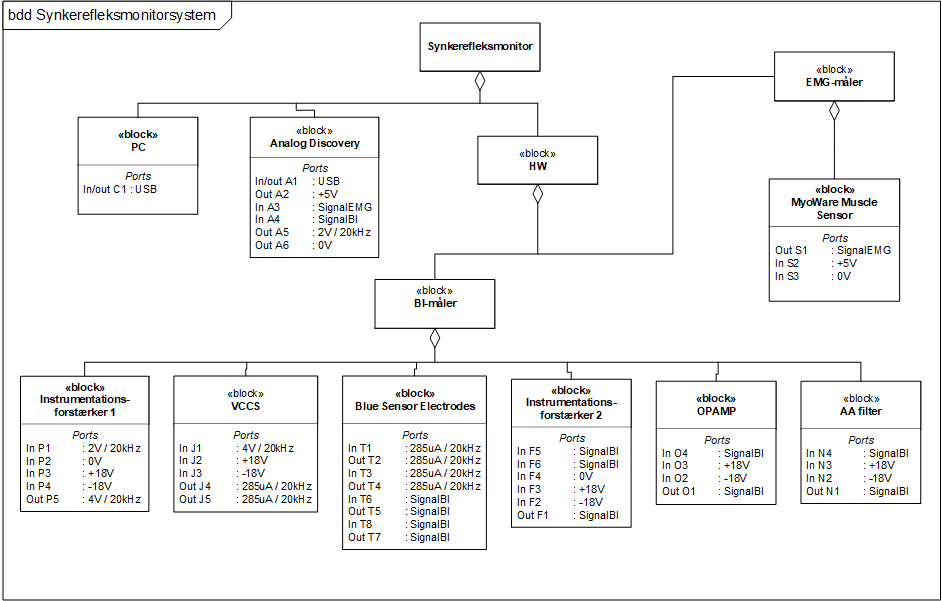
\includegraphics[width=\linewidth]
{Figure/BDD2}}
\caption{Figuren viser de enkelte komponenter, som hardware-delen består af. Overordnet består hardwaren af en Bioimpedansmåler og EMG-måler og en enhed, som bruges til at forsyne  målerapparaterne. DAQ'en anvendes som dataopsamlingsenhed.}
\label{figbdd}
\end{figure}

\section{Internal blok diagram}

Det interne blokdiagram på \ref{ibdfigur} viser den interne struktur og kommunikation mellem delsystemer. Figur \ref{ibdfigur} indeholder to uafhængige blokke med navnene BI-måler og EMG-måler. De to måleapparater kommunikerer med Analog Discovery og en PC. For BI-målerens vedkommende starter kommunikationsflowet med at Analog Discovery'en sender to \textbf{2V} AC spænding til den første forstærker i BI-måler blokken. Forstærker 1 forstærker de \textbf{2V} med faktor 2. Det forstærket signal sendes videre til strømgeneratoren, VCCS, som på baggrund af det indkommende spænding producerer en konstant strøm på \textbf{0,5mA}. Strømen sendes videre til et måleobjekt via. to elektroder, kaldet Blue Sensor Electrodes.       Yderligere to elektroder påsættes på måleobjektet for at måle en spændingsforskel. Denne spændingsforskel ligger i millivolt området og kræver at blive forstærket. Denne forstærkning foregår over trin. Til formålet anvendes en instrumentationsforstærker efterfulgt af en operationsforstærker. Det forstærker signal sendes videre til et anti-aliaseringsfilter, der dæmper frekvenskomponenter over \textbf{Nyquist-frekvensen}. Tilslut sendes signalet til en dataopsamlingsenhed, kaldet DAQ NI USB-6259, der sender det opsamlede signal videre til en PC for at blive analyseret og vist. Delsystemerne forstærker 1, 2 og AA filteret forsynes med en eksitationsspænding på $ \pm  $\textbf{18V}. \\

EMG-blokken består en Myoware Muscle Sensor og to elektroder, der måler spændingsfaldet over et valgt segment på et måleobjekt. Det målte signal sendes til en PC for at blive vist. Myoware Muscle Sensorens eksitationsspænding på \textbf{5V} på  kommer fra Analog Discovery.   
					\textbf{INDSÆT EN BLOK OM ELNETET} 
\begin{figure}[H]
\centering
{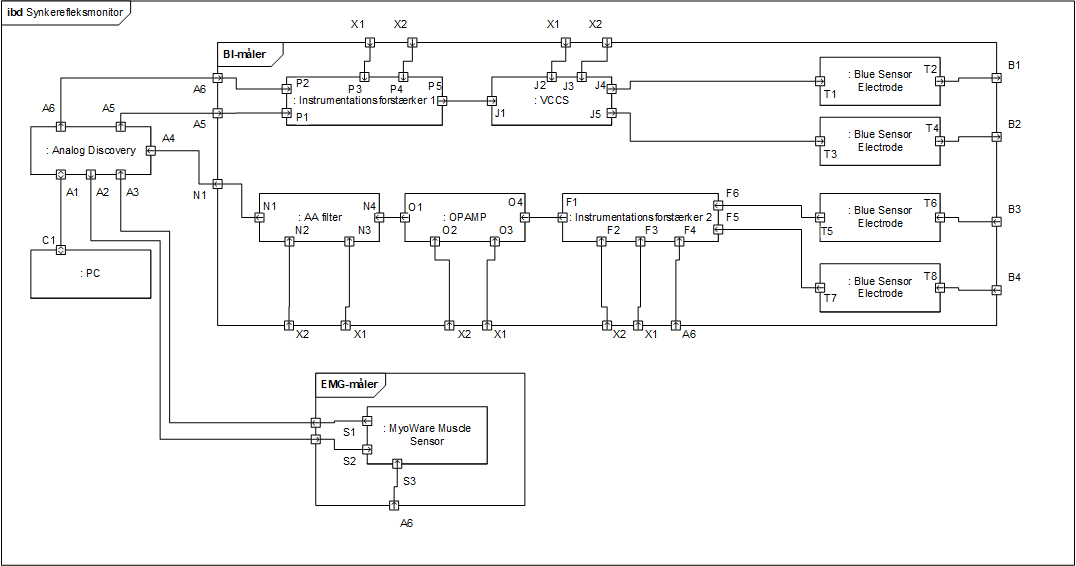
\includegraphics[width=\linewidth]
{Figure/IBD2}}
\caption{Figuren viser et internt blokdiagram, der illustrer den interne relation og signalflow mellem delsystemer. Overordnet set indeholder diagrammet to hovedblokke med hver deres subkomponenter. Den ene af de store blokke repræsenter en bioimpedansmåler-apparat og den anden blok repræsenter en elektromyografi-apparat }
\label{ibdfigur}
\end{figure}

\section{Blokbeskrivelse} \label{blokbesk}
Nedenstående tabel viser den enkelte blokes funktion, signaltype og port navn, som indgår i IBD'et på figur \ref{ibdfigur}.

\begin{table} [H]
  \centering

\begin{tabular}  {|p{3cm}|p{4cm}|p{1cm}|p{1.5cm}|p{3.8cm}| }

\hline
	
	\textbf{Blok-navn} & \textbf{Funktionbeskrivelse}  & \textbf{Port} & \textbf{Signaler} & \textbf{Kommentar} \\ \cline{3-5} \hline
	
PC & Behandler input fra Analog Discovery.  &  C1 & bit(USB)  & Interfacekommunikation  \\ \cline{3-5}
	 &  & C2 & Graf & Impedans og tid \\ 
	 
	 \hline
	 
	 
Analog Discovery  & Forsyner MyoWare Muscle Sensor og Forstærker 1. Den fungerer også som  Analog-til-digital-konverter.  &  A1 & 2V & Udgangsspænding    \\ \cline{3-5}
	 &  & A2 & bit(seriel) & Indgangsspænding \\ \cline{3-5}
	 &  & A3 & bit(USB)  & Interfacekommunikation \\
 \cline{3-5}
	 &  & A4 & bit(seriel)  & Indgangsspænding 	 
	 \\
 \cline{3-5}
	 &  & A5 & 5V  & Eksitationsspænding 	 	 
	 
	 
	  \\ \hline	  
	 
		 
 Forstærker 1 & Forstærker 2V fra Analog Discovery til 4V   &  P1 & 2V & Indgangsspænding   \\ \cline{3-5}
	 &  & P2 & $   ${-18V}  & Eksitationsspænding \\ \cline{3-5}
	 &  & P3 & 4V  & Udgangsspænding   \\ 
	\cline{3-5}
	 &  & P4 & $   ${18V}  & Eksitationsspænding   
	 
	  \\ \hline	 	
	 
	 
Strømgenerator  & Genererer en konstant strøm &  J1 &$   ${18V} & Eksitationsspænding    \\ \cline{3-5}
	 &  & J2 & 4V  & Indgangsspænding \\ \cline{3-5}
	 &  & J3 & $ \pm  $\textbf{0.5mA}  & Udgangsstrøm  \\ \cline{3-5}
	
	 &  & J4 & $  ${-18V}  & Eksitationsspænding 	 
	 
	   \\ \hline 
	 
	 
 Forstærker 2 & Forstærker biosignal fra et måleobjekt   &  F1 & mV & Indgangsspænding     \\ \cline{3-5}
	 &  & F2 & $  ${18V}  & Eksitationsspænding \\ \cline{3-5}
	 &  & F3 & V  & Udgangsspænding  \\ \cline{3-5}
	 &  & F4 & $  ${-18V}  & Eksitationsspænding
	 
	   \\ \hline
	 
	 
4 x Blue Sensor Electrodes & Transporterer strøm til et måleobjekt og måler biosignal fra et måleobjekt.  &  T1 & uA & Udgangsstrøm  \\ \cline{3-5}
	 &  & T2 & uA & Udgangsstrøm \\ \cline{3-5} 
	 &  & T3 & mV & Biopotentiale \\ \cline{3-5} 
	 &  & T4 & mV & Biopotentiale \\ \cline{3-5}  \hline
	 
	 
	  OPAMP & Forstærker signalet fra forstærker 2
	 &  O1 & V & Indgangsspænding     \\ \cline{3-5}
	 &  & O2 & $  ${18V}  & Eksitationsspænding \\ \cline{3-5}
	 &  & O3 & V  & Udgangsspænding  \\ \cline{3-5}
	 &  & O4 & $  ${-18V}  & Eksitationsspænding
	 
	   \\ \hline
	 
 \end{tabular}
 
\end{table}

\pagebreak

\begin{table} [H]
  \centering

\begin{tabular}  {|p{3cm}|p{4cm}|p{1cm}|p{1.5cm}|p{3.8cm}| }

\hline

AA filter & Bruges til at undgå aliasering.  &  N1 & V & Indgangsspænding  \\ \cline{3-5}
	 &  & N2 & $  ${18V} & Eksitationsspænding \\ \cline{3-5} 
	 &  & N3 & V & Udgangsspænding \\ \cline{3-5} 
	 &  & N4 & $  ${-18V} & Eksitationsspænding \\ \cline{3-5} 
	 
	 \hline
	 

MyoWare Muscle Sensor & Behandler EMG input fra et måleobjekt 		 &  S1 & mV & Biopotentiale  \\ \cline{3-5}
	 &  & S2 & bit(seriel) & Biopotentiale \\ \cline{3-5} 
	 &  & S3 & 5V & Eksitationsspænding \\ \cline{3-5} \hline
	 
	 
2x Kendall electrodes & Transporterer EMG signal fra et måleobjekt  &  L1 & mV & Biopotentiale  \\ \cline{3-5}
	 &  & L2 & mV & Biopotentiale \\ \cline{3-5} \hline
	 

\end{tabular}
 \caption{Figuren giver overblik over blok navn, blok funktionn og signaltype af de komponenter, som indgår i det interne blokdiagram på figur \ref{ibdfigur}} \label{tab:Sigbeskriv.}
\end{table}

\textbf{Husk den anden Tabel}
\chapter{Software} \label{swafsnit}
\section{Script session diagram}

Dette afsnit omhandler strukturering af den  software, som anvendes til analysering og visning af bioimpedans- og EMG målinger. Design af softwaren er drevet af de usecases, som er beskrevet i afsnittet systembeskrivelse. På baggrund af disse usecases udformes en script session diagram, som indeholder blokke, der hver repræsenterer en funktion/metode som udfører en bestemt opgave. 
I dette projekt anvendes Matlab til at implementere systemets software. Matlab er ikke et objekt orienteret programmeringssprog, men derimod scriptsprog. Dette gør at at det bliver vanskeligt at anvende diagrammer, som er brugt til at strukturere objekt orienteret programmeringskoder. For at skabe en form for struktur i arkitekturen er der lavet et alternativt diagram kaldet   Matlab script session diagram. Funktionaliteter som ønskes implementeret i Matlab kodes som funktioner. Da vi ønsker at implementere Matlab GUI med kontroller i dette projekt skrives koden til disse kontroller i funktioner. Kontrollerne kan være en knap, tekstfelt eller tekstboks. I stedet for at kode alle funktioner i én scriptfil tildeles hver funktionen sin egen script session. Hver script session omtales som et objekt,der udfører en bestemt opgave, samt kan interagerer med andre objekter. På den måde er der forsøgt at lave et system/diagram som giver overblik over de funktioner som indgår i software-delen. Konkret fungerer softwaren ved at et sundhedspersonalet initialiserer koden ved at trykke på knapperne ’Start EMG-måling' og ’Start BI-måling’. Denne initiering medfører at koden, som ligger bag begge knapper udføreres og der foretages to målinger. Disse målinger gemmes i .mat-filer som gemmes lokalt på PC’en. For at analysere og vise målingerne  uploades de gemte filer til softwaren.  


\begin{figure}[H] 
\centering
{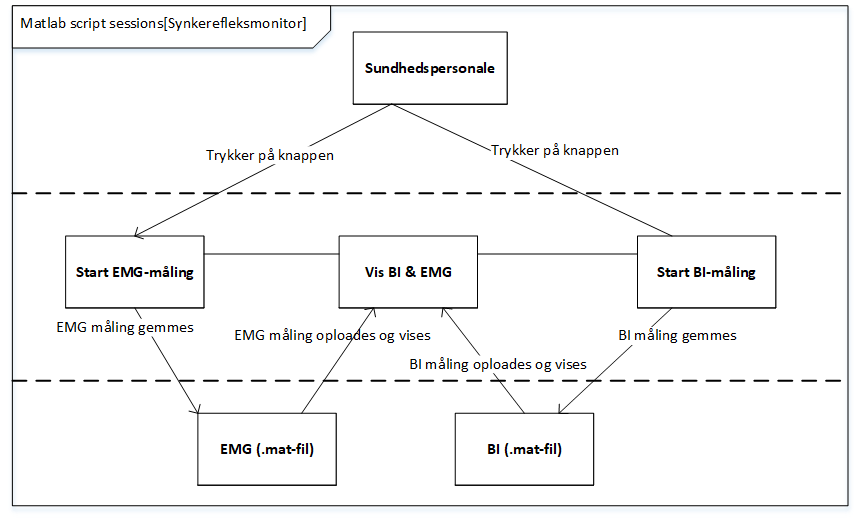
\includegraphics[width=\linewidth]
{Figure/ScriptSessionDia}}
\caption{Figuren viser de tre lag som koden er inddelt. Kode eksekveringen initialiseres af et sundhedspersonale ved at trykke på knapperne ’Start EMG-måling’ og ’Start BI-måling. Efterfølgende foretages en måling, som gemmes lokal i PC'en. Tilslut uploades de gemte målinger for at blive analyseret og vist.}
\label{figScrip}
\end{figure}



\citep{Aroom2009}
\bibliography{library}
\end{document}